% Options for packages loaded elsewhere
% Options for packages loaded elsewhere
\PassOptionsToPackage{unicode}{hyperref}
\PassOptionsToPackage{hyphens}{url}
\PassOptionsToPackage{dvipsnames,svgnames,x11names}{xcolor}
%
\documentclass[
  letterpaper,
  DIV=11,
  numbers=noendperiod]{scrartcl}
\usepackage{xcolor}
\usepackage{amsmath,amssymb}
\setcounter{secnumdepth}{-\maxdimen} % remove section numbering
\usepackage{iftex}
\ifPDFTeX
  \usepackage[T1]{fontenc}
  \usepackage[utf8]{inputenc}
  \usepackage{textcomp} % provide euro and other symbols
\else % if luatex or xetex
  \usepackage{unicode-math} % this also loads fontspec
  \defaultfontfeatures{Scale=MatchLowercase}
  \defaultfontfeatures[\rmfamily]{Ligatures=TeX,Scale=1}
\fi
\usepackage{lmodern}
\ifPDFTeX\else
  % xetex/luatex font selection
\fi
% Use upquote if available, for straight quotes in verbatim environments
\IfFileExists{upquote.sty}{\usepackage{upquote}}{}
\IfFileExists{microtype.sty}{% use microtype if available
  \usepackage[]{microtype}
  \UseMicrotypeSet[protrusion]{basicmath} % disable protrusion for tt fonts
}{}
\makeatletter
\@ifundefined{KOMAClassName}{% if non-KOMA class
  \IfFileExists{parskip.sty}{%
    \usepackage{parskip}
  }{% else
    \setlength{\parindent}{0pt}
    \setlength{\parskip}{6pt plus 2pt minus 1pt}}
}{% if KOMA class
  \KOMAoptions{parskip=half}}
\makeatother
% Make \paragraph and \subparagraph free-standing
\makeatletter
\ifx\paragraph\undefined\else
  \let\oldparagraph\paragraph
  \renewcommand{\paragraph}{
    \@ifstar
      \xxxParagraphStar
      \xxxParagraphNoStar
  }
  \newcommand{\xxxParagraphStar}[1]{\oldparagraph*{#1}\mbox{}}
  \newcommand{\xxxParagraphNoStar}[1]{\oldparagraph{#1}\mbox{}}
\fi
\ifx\subparagraph\undefined\else
  \let\oldsubparagraph\subparagraph
  \renewcommand{\subparagraph}{
    \@ifstar
      \xxxSubParagraphStar
      \xxxSubParagraphNoStar
  }
  \newcommand{\xxxSubParagraphStar}[1]{\oldsubparagraph*{#1}\mbox{}}
  \newcommand{\xxxSubParagraphNoStar}[1]{\oldsubparagraph{#1}\mbox{}}
\fi
\makeatother

\usepackage{color}
\usepackage{fancyvrb}
\newcommand{\VerbBar}{|}
\newcommand{\VERB}{\Verb[commandchars=\\\{\}]}
\DefineVerbatimEnvironment{Highlighting}{Verbatim}{commandchars=\\\{\}}
% Add ',fontsize=\small' for more characters per line
\usepackage{framed}
\definecolor{shadecolor}{RGB}{241,243,245}
\newenvironment{Shaded}{\begin{snugshade}}{\end{snugshade}}
\newcommand{\AlertTok}[1]{\textcolor[rgb]{0.68,0.00,0.00}{#1}}
\newcommand{\AnnotationTok}[1]{\textcolor[rgb]{0.37,0.37,0.37}{#1}}
\newcommand{\AttributeTok}[1]{\textcolor[rgb]{0.40,0.45,0.13}{#1}}
\newcommand{\BaseNTok}[1]{\textcolor[rgb]{0.68,0.00,0.00}{#1}}
\newcommand{\BuiltInTok}[1]{\textcolor[rgb]{0.00,0.23,0.31}{#1}}
\newcommand{\CharTok}[1]{\textcolor[rgb]{0.13,0.47,0.30}{#1}}
\newcommand{\CommentTok}[1]{\textcolor[rgb]{0.37,0.37,0.37}{#1}}
\newcommand{\CommentVarTok}[1]{\textcolor[rgb]{0.37,0.37,0.37}{\textit{#1}}}
\newcommand{\ConstantTok}[1]{\textcolor[rgb]{0.56,0.35,0.01}{#1}}
\newcommand{\ControlFlowTok}[1]{\textcolor[rgb]{0.00,0.23,0.31}{\textbf{#1}}}
\newcommand{\DataTypeTok}[1]{\textcolor[rgb]{0.68,0.00,0.00}{#1}}
\newcommand{\DecValTok}[1]{\textcolor[rgb]{0.68,0.00,0.00}{#1}}
\newcommand{\DocumentationTok}[1]{\textcolor[rgb]{0.37,0.37,0.37}{\textit{#1}}}
\newcommand{\ErrorTok}[1]{\textcolor[rgb]{0.68,0.00,0.00}{#1}}
\newcommand{\ExtensionTok}[1]{\textcolor[rgb]{0.00,0.23,0.31}{#1}}
\newcommand{\FloatTok}[1]{\textcolor[rgb]{0.68,0.00,0.00}{#1}}
\newcommand{\FunctionTok}[1]{\textcolor[rgb]{0.28,0.35,0.67}{#1}}
\newcommand{\ImportTok}[1]{\textcolor[rgb]{0.00,0.46,0.62}{#1}}
\newcommand{\InformationTok}[1]{\textcolor[rgb]{0.37,0.37,0.37}{#1}}
\newcommand{\KeywordTok}[1]{\textcolor[rgb]{0.00,0.23,0.31}{\textbf{#1}}}
\newcommand{\NormalTok}[1]{\textcolor[rgb]{0.00,0.23,0.31}{#1}}
\newcommand{\OperatorTok}[1]{\textcolor[rgb]{0.37,0.37,0.37}{#1}}
\newcommand{\OtherTok}[1]{\textcolor[rgb]{0.00,0.23,0.31}{#1}}
\newcommand{\PreprocessorTok}[1]{\textcolor[rgb]{0.68,0.00,0.00}{#1}}
\newcommand{\RegionMarkerTok}[1]{\textcolor[rgb]{0.00,0.23,0.31}{#1}}
\newcommand{\SpecialCharTok}[1]{\textcolor[rgb]{0.37,0.37,0.37}{#1}}
\newcommand{\SpecialStringTok}[1]{\textcolor[rgb]{0.13,0.47,0.30}{#1}}
\newcommand{\StringTok}[1]{\textcolor[rgb]{0.13,0.47,0.30}{#1}}
\newcommand{\VariableTok}[1]{\textcolor[rgb]{0.07,0.07,0.07}{#1}}
\newcommand{\VerbatimStringTok}[1]{\textcolor[rgb]{0.13,0.47,0.30}{#1}}
\newcommand{\WarningTok}[1]{\textcolor[rgb]{0.37,0.37,0.37}{\textit{#1}}}

\usepackage{longtable,booktabs,array}
\newcounter{none} % for unnumbered tables
\usepackage{calc} % for calculating minipage widths
% Correct order of tables after \paragraph or \subparagraph
\usepackage{etoolbox}
\makeatletter
\patchcmd\longtable{\par}{\if@noskipsec\mbox{}\fi\par}{}{}
\makeatother
% Allow footnotes in longtable head/foot
\IfFileExists{footnotehyper.sty}{\usepackage{footnotehyper}}{\usepackage{footnote}}
\makesavenoteenv{longtable}
\usepackage{graphicx}
\makeatletter
\newsavebox\pandoc@box
\newcommand*\pandocbounded[1]{% scales image to fit in text height/width
  \sbox\pandoc@box{#1}%
  \Gscale@div\@tempa{\textheight}{\dimexpr\ht\pandoc@box+\dp\pandoc@box\relax}%
  \Gscale@div\@tempb{\linewidth}{\wd\pandoc@box}%
  \ifdim\@tempb\p@<\@tempa\p@\let\@tempa\@tempb\fi% select the smaller of both
  \ifdim\@tempa\p@<\p@\scalebox{\@tempa}{\usebox\pandoc@box}%
  \else\usebox{\pandoc@box}%
  \fi%
}
% Set default figure placement to htbp
\def\fps@figure{htbp}
\makeatother





\setlength{\emergencystretch}{3em} % prevent overfull lines

\providecommand{\tightlist}{%
  \setlength{\itemsep}{0pt}\setlength{\parskip}{0pt}}



 


\KOMAoption{captions}{tableheading}
\makeatletter
\@ifpackageloaded{tcolorbox}{}{\usepackage[skins,breakable]{tcolorbox}}
\@ifpackageloaded{fontawesome5}{}{\usepackage{fontawesome5}}
\definecolor{quarto-callout-color}{HTML}{909090}
\definecolor{quarto-callout-note-color}{HTML}{0758E5}
\definecolor{quarto-callout-important-color}{HTML}{CC1914}
\definecolor{quarto-callout-warning-color}{HTML}{EB9113}
\definecolor{quarto-callout-tip-color}{HTML}{00A047}
\definecolor{quarto-callout-caution-color}{HTML}{FC5300}
\definecolor{quarto-callout-color-frame}{HTML}{acacac}
\definecolor{quarto-callout-note-color-frame}{HTML}{4582ec}
\definecolor{quarto-callout-important-color-frame}{HTML}{d9534f}
\definecolor{quarto-callout-warning-color-frame}{HTML}{f0ad4e}
\definecolor{quarto-callout-tip-color-frame}{HTML}{02b875}
\definecolor{quarto-callout-caution-color-frame}{HTML}{fd7e14}
\makeatother
\makeatletter
\@ifpackageloaded{caption}{}{\usepackage{caption}}
\AtBeginDocument{%
\ifdefined\contentsname
  \renewcommand*\contentsname{Table of contents}
\else
  \newcommand\contentsname{Table of contents}
\fi
\ifdefined\listfigurename
  \renewcommand*\listfigurename{List of Figures}
\else
  \newcommand\listfigurename{List of Figures}
\fi
\ifdefined\listtablename
  \renewcommand*\listtablename{List of Tables}
\else
  \newcommand\listtablename{List of Tables}
\fi
\ifdefined\figurename
  \renewcommand*\figurename{Figure}
\else
  \newcommand\figurename{Figure}
\fi
\ifdefined\tablename
  \renewcommand*\tablename{Table}
\else
  \newcommand\tablename{Table}
\fi
}
\@ifpackageloaded{float}{}{\usepackage{float}}
\floatstyle{ruled}
\@ifundefined{c@chapter}{\newfloat{codelisting}{h}{lop}}{\newfloat{codelisting}{h}{lop}[chapter]}
\floatname{codelisting}{Listing}
\newcommand*\listoflistings{\listof{codelisting}{List of Listings}}
\makeatother
\makeatletter
\makeatother
\makeatletter
\@ifpackageloaded{caption}{}{\usepackage{caption}}
\@ifpackageloaded{subcaption}{}{\usepackage{subcaption}}
\makeatother
\usepackage{bookmark}
\IfFileExists{xurl.sty}{\usepackage{xurl}}{} % add URL line breaks if available
\urlstyle{same}
\hypersetup{
  pdftitle={rENM Framework User Manual},
  pdfauthor={John L. Schnase},
  colorlinks=true,
  linkcolor={blue},
  filecolor={Maroon},
  citecolor={Blue},
  urlcolor={Blue},
  pdfcreator={LaTeX via pandoc}}


\title{rENM Framework User Manual}
\usepackage{etoolbox}
\makeatletter
\providecommand{\subtitle}[1]{% add subtitle to \maketitle
  \apptocmd{\@title}{\par {\large #1 \par}}{}{}
}
\makeatother
\subtitle{Version 0.1.0}
\author{John L. Schnase}
\date{2026-06-21}
\begin{document}
\maketitle

\renewcommand*\contentsname{Table of contents}
{
\setcounter{tocdepth}{3}
\tableofcontents
}

\newpage{}

\begin{tcolorbox}[enhanced jigsaw, arc=.35mm, bottomrule=.15mm, breakable, colback=white, colframe=quarto-callout-caution-color-frame, left=2mm, leftrule=.75mm, opacityback=0, rightrule=.15mm, toprule=.15mm]

\textbf{\emph{Content is subject to ongoing revision and periodic
updates \ldots{}}}

\end{tcolorbox}

\section{Introduction}\label{introduction}

The rENM Framework is a modular suite of R packages designed to support
the development and analysis of retrospective ecological niche models
(rENMs). Retrospective ecological niche modeling integrates historical
species occurrence records with historical environmental data to
reconstruct the spatio-temporal dynamics of species' responses to
changing environmental conditions.

By revealing long-term patterns, rENMs provide an empirical basis for
addressing biological questions and assessing both the current and
future conservation status of species. Rather than treating ecological
niche models as static representations, the rENM Framework uses
time-structured modeling to reveal:

\begin{itemize}
\tightlist
\item
  Long-term trends in climatic suitability for a species
\item
  Acceleration and deceleration of those trends
\item
  Directional change in suitability and shifts in the
  suitability-weighted geographic center of a species' climatic niche
\item
  Changes in the relative importance of environmental predictors across
  decades
\item
  Bioclimatic velocity
\item
  Hotspots of accelerating suitability decline
\end{itemize}

Although this analytical approach is broadly applicable across taxa, the
current implementation of the rENM Framework is designed to investigate
climate-driven dynamics in North American bird species. The framework
spans 45 years (1980--2024), leveraging citizen science observations
from the Cornell Lab of Ornithology's eBird database alongside
environmental data derived from NASA's Modern-Era Retrospective Analysis
for Research and Applications, Version 2 (MERRA-2).

This manual guides users through the rENM modeling and analysis
workflow. Detailed documentation for individual functions is available
within the respective package manuals. Additional information about this
work can be found in the Appendix A publications and the project's
GitHub repository at: \url{https://github.com/rENM-Framework}.

The rENM Framework is an active research platform under ongoing
development. It is provided for educational and research purposes only
and is distributed without formal technical support. Feedback and
contributions are welcome.

Thank you for your interest.

John Schnase\\
rENM.Framework@gmail.com

\newpage{}

\section{The rENM Workflow}\label{the-renm-workflow}

\pandocbounded{
\includegraphics[keepaspectratio]{images/clipboard-2962903405.png}}

The rENM processing pipeline consists of five core steps, including an
optional, experimental GenAI-mediated interpretation step. One way to
engage this workflow is by using this Quarto Markdown (.qmd) document as
an interactive user manual. It becomes a reproducible, executable
scientific document that combines code, results, and narrative into a
single, renderable file.

\subsection{Using the Quarto document}\label{using-the-quarto-document}

After initially configuring your host environment and RStudio
environment (see \emph{Configuring the Host Environment} and
\emph{Configuring the RStudio Environment} below), set the species
banding code and step through each section in sequence, reading the
narrative description of each processing step and executing the
accompanying code block before moving on. This mode is well suited to
users who are learning the framework.

You may also copy the \emph{rENM-Framework-User-Manual.qmd} file, rename
it, and use it as a customized, reproducible analysis notebook for your
own species or study system. Because the document combines function
calls, parameter settings, and narrative in a single file, it can serve
alongside a run's output directory as a complete and portable record of
the analysis.

Finally, from the RStudio \textbf{\texttt{Run}} drop-down menu, select
\emph{Restart R and Run All Chunks} to execute the entire workflow
automatically, without stepping through it manually.

\subsection{Automated scripting}\label{automated-scripting}

If you prefer not to run an rENM analysis step by step, you can execute
the full pipeline from the RStudio console with a single function call.
For example: \texttt{rENM("CASP")}. Enter \texttt{?rENM} in the RStudio
console for details.

\subsection{Document rendering
options}\label{document-rendering-options}

If you use the \emph{rENM-Framework-User-Manual.qmd} file as a template
for your own species or study system, RStudio's Quarto rendering engine
can convert it to multiple output formats from the \texttt{Render}
drop-down menu, including HTML, PDF, and Microsoft Word (DOCX). A
Jupyter Notebook (IPYNB) version can also be rendered, producing a
notebook that executes the same rENM Framework functions in an R kernel
environment and making the workflow accessible to users who prefer the
Jupyter interface without requiring any modification to the underlying R
code.

\section{System Requirements}\label{system-requirements}

The rENM Framework requires R (≥ 4.1.0) and two external software
dependencies, LibreOffice and Chrome or Chromium, that must be installed
separately before the full pipeline can run. The Framework has been
developed and tested on macOS and is expected to be compatible with
Linux. Windows users may experience longer run times due to limited
support for parallel processing on that platform. All R package
dependencies are installed automatically when you install the framework
packages from GitHub (see \emph{Installing the Framework Packages}
below).

\subsection{R package dependencies}\label{r-package-dependencies}

Two framework packages pull in heavy R dependencies worth anticipating
before installation:

\begin{itemize}
\tightlist
\item
  \textbf{\texttt{rENM.model}} depends on \texttt{sdm}, which requires
  \texttt{randomForest}, \texttt{gbm}, and \texttt{earth} as modeling
  back-ends. These are installed on first use.
\item
  \textbf{\texttt{rENM.analysis}} depends on \texttt{rstanarm} for
  Bayesian trend estimation. \texttt{rstanarm} is large and may take
  several minutes to compile on first install.
\end{itemize}

The \texttt{rENM.reports} package uses \texttt{webshot2},
\texttt{pagedown}, and \texttt{chromote} for PNG and PDF rendering of
summary tables. These are optional and must be installed separately (see
\emph{Chrome or Chromium} below). The Excel (XLSX) output from summary
table functions is always written regardless of whether these packages
are installed.

\subsection{LibreOffice}\label{libreoffice}

\texttt{rENM.ai::render\_ai\_docx()} converts AI-generated DOCX reports
to PDF using LibreOffice in headless mode. LibreOffice must be installed
before using that function.

Download from \url{https://www.libreoffice.org}. On macOS, LibreOffice
installs to \texttt{/Applications} but its \texttt{soffice} binary is
not added to \texttt{PATH} automatically. Run this once in Terminal
after installing:

\begin{Shaded}
\begin{Highlighting}[]
\FunctionTok{sudo}\NormalTok{ ln }\AttributeTok{{-}s}\NormalTok{ /Applications/LibreOffice.app/Contents/MacOS/soffice /usr/local/bin/soffice}
\end{Highlighting}
\end{Shaded}

On Linux, install via your package manager (e.g.,
\texttt{apt\ install\ libreoffice}); \texttt{soffice} is placed on
\texttt{PATH} automatically. If LibreOffice is absent when
\texttt{render\_ai\_docx()} is called, a clear error message is
displayed with installation instructions.

\subsection{Chrome or Chromium}\label{chrome-or-chromium}

\texttt{rENM.reports} renders summary tables as PNG and PDF files by
driving a headless Chrome browser via the \texttt{chromote},
\texttt{webshot2}, and \texttt{pagedown} packages. Install these R
packages first:

\begin{Shaded}
\begin{Highlighting}[]
\FunctionTok{install.packages}\NormalTok{(}\FunctionTok{c}\NormalTok{(}\StringTok{"chromote"}\NormalTok{, }\StringTok{"webshot2"}\NormalTok{, }\StringTok{"pagedown"}\NormalTok{))}
\end{Highlighting}
\end{Shaded}

Then verify Chrome is found before running the pipeline:

\begin{Shaded}
\begin{Highlighting}[]
\NormalTok{chromote}\SpecialCharTok{::}\FunctionTok{find\_chrome}\NormalTok{()}
\end{Highlighting}
\end{Shaded}

If that call throws an error, install Google Chrome from
\url{https://www.google.com/chrome/} and re-run
\texttt{chromote::find\_chrome()} to confirm. If Chrome is unavailable
at runtime, PNG and PDF outputs from the summary table functions are
silently skipped with a console note; the XLSX output is always written
regardless.

\subsection{Troubleshooting package
installation}\label{troubleshooting-package-installation}

The rENM Framework uses \texttt{paletteer} for color scales in several
plotting functions. If you encounter an unexpected ``package not found''
error during a plotting step, check whether a \texttt{paletteer}-based
color scale is the source. The missing package will be named in the
error message; install it with \texttt{install.packages()} and re-run
the function.

\section{Configuring the Host
Environment}\label{configuring-the-host-environment}

The rENM Framework relies on a simple, standardized filesystem
structure. At the top level is a project directory containing a
\texttt{data} subdirectory for input datasets and a \texttt{runs}
subdirectory where model outputs and analysis results are written. The
initial setup creates this structure, installs the example dataset, and
creates a symbolic link that points to it from the \texttt{data}
subdirectory.

\begin{verbatim}
PROJECT_DIRECTORY/
|___ data -> (symbolic link to dataset in use)
|___ rENM-Framework-v0.1.0-example-data/...
|___ rENM-Framework-v0.1.0-extended-data/...
|___ my_input_data/...
|___ runs/...
\end{verbatim}

You only need to configure your host environment once. The examples
below assume a macOS or Linux environment using the Bash shell. If you
prefer to run these commands outside of RStudio, equivalent scripts are
available at \url{https://github.com/rENM-Framework/rENM-scripts}.

\subsection{Creating the project
directory}\label{creating-the-project-directory}

Create the project directory and the \texttt{runs} subdirectory from a
terminal window. The name \texttt{rENMtest} is used here for
illustration; choose a name that fits your own workflow.

\begin{Shaded}
\begin{Highlighting}[]
\CommentTok{\#!/usr/bin/env bash}

\CommentTok{\# set project directory name}
\VariableTok{PROJECT\_DIRECTORY}\OperatorTok{=}\StringTok{"}\VariableTok{$HOME}\StringTok{/rENMtest"}

\CommentTok{\# create initial directory structure}
\FunctionTok{mkdir} \AttributeTok{{-}p} \StringTok{"}\VariableTok{$PROJECT\_DIRECTORY}\StringTok{"}
\FunctionTok{mkdir} \AttributeTok{{-}p} \StringTok{"}\VariableTok{$PROJECT\_DIRECTORY}\StringTok{/runs"}
\end{Highlighting}
\end{Shaded}

\subsection{Installing the example
dataset}\label{installing-the-example-dataset}

The example dataset includes occurrence records for three focal species:
Brown-capped Rosy-Finch (\emph{Leucosticte australis}; BCRF), Cassin's
Sparrow (\emph{Peucaea cassinii}; CASP), and Greater Roadrunner
(\emph{Geococcyx californianus}; GRRO). Also included are 14 MERRA-2 and
MERRAclim-2 environmental variables, shapefiles for state boundaries and
species ranges, and a catalog of the dataset's contents. The dataset is
approximately 725 MB.

The dataset is archived on Zenodo and downloaded automatically by the
commands below. Make sure your current working directory is the project
directory you created above, then run the following commands from a
terminal window to download and install it:

\begin{Shaded}
\begin{Highlighting}[]
\CommentTok{\#!/usr/bin/env bash}

\CommentTok{\# set project directory name (same as above)}
\VariableTok{PROJECT\_DIRECTORY}\OperatorTok{=}\StringTok{"}\VariableTok{$HOME}\StringTok{/rENMtest"}
\BuiltInTok{cd} \StringTok{"}\VariableTok{$\{PROJECT\_DIRECTORY\}}\StringTok{"}

\CommentTok{\# download and unzip example dataset}
\VariableTok{DATA\_URL}\OperatorTok{=}\StringTok{"https://zenodo.org/records/20750253/files/rENM{-}Framework{-}v0.1.0{-}example{-}data.zip"}
\VariableTok{ZIP\_FILE}\OperatorTok{=}\StringTok{"rENM{-}Framework{-}v0.1.0{-}example{-}data.zip"}
\ExtensionTok{curl} \AttributeTok{{-}L} \AttributeTok{{-}o} \StringTok{"}\VariableTok{$\{ZIP\_FILE\}}\StringTok{"} \StringTok{"}\VariableTok{$\{DATA\_URL\}}\StringTok{"}
\FunctionTok{unzip} \AttributeTok{{-}o} \StringTok{"}\VariableTok{$\{ZIP\_FILE\}}\StringTok{"}

\CommentTok{\# create symbolic link}
\FunctionTok{ln} \AttributeTok{{-}sfn}\NormalTok{ rENM{-}Framework{-}v0.1.0{-}example{-}data data}

\CommentTok{\# clean up}
\FunctionTok{rm} \AttributeTok{{-}rf}\NormalTok{ \_\_MACOSX}
\FunctionTok{rm} \AttributeTok{{-}f} \StringTok{"}\VariableTok{$\{ZIP\_FILE\}}\StringTok{"}
\end{Highlighting}
\end{Shaded}

\section{Configuring the RStudio
Environment}\label{configuring-the-rstudio-environment}

All subsequent work is performed in RStudio using R. Begin by specifying
the location of the project directory you created in the previous
section. This allows both RStudio and the rENM Framework to locate and
manage project files consistently across sessions.

\subsection{Setting the project directory
location}\label{setting-the-project-directory-location}

The following command writes the project directory path to your
\texttt{.Renviron} file, making it available in every future R session.
Run it once during initial setup, then leave it commented out.

\begin{Shaded}
\begin{Highlighting}[]
\CommentTok{\# \# set the location of the project directory}
\CommentTok{\# write(}
\CommentTok{\#   paste0(\textquotesingle{}RENM\_PROJECT\_DIR="\textquotesingle{}, file.path(Sys.getenv("HOME"), "rENMtest"), \textquotesingle{}"\textquotesingle{}),}
\CommentTok{\#   file = "\textasciitilde{}/.Renviron",}
\CommentTok{\#   append = TRUE}
\CommentTok{\# )}
\CommentTok{\# \# reload (or restart R)}
\CommentTok{\# readRenviron("\textasciitilde{}/.Renviron")}
\CommentTok{\# Sys.getenv("RENM\_PROJECT\_DIR")}
\end{Highlighting}
\end{Shaded}

For single-session use, you can set the project directory with
\texttt{options(rENM.project\_dir\ =\ ...)} instead of configuring
\texttt{.Renviron}. See \texttt{?rENM\_project\_dir} for details.

\subsection{Installing the framework
packages}\label{installing-the-framework-packages}

Install the rENM Framework packages from GitHub. The \texttt{remotes}
package handles installation from remote repositories and is all that is
needed for this step. Install the packages in the order shown, with the
top-level \texttt{rENM} orchestration package last.

\begin{Shaded}
\begin{Highlighting}[]
\CommentTok{\# \# install rENM Framework packages from the GitHub repository}
\CommentTok{\# install.packages("remotes")}
\CommentTok{\# remotes::install\_github("rENM{-}Framework/rENM.core")}
\CommentTok{\# remotes::install\_github("rENM{-}Framework/rENM.data")}
\CommentTok{\# remotes::install\_github("rENM{-}Framework/rENM.model")}
\CommentTok{\# remotes::install\_github("rENM{-}Framework/rENM.analysis")}
\CommentTok{\# remotes::install\_github("rENM{-}Framework/rENM.ai")}
\CommentTok{\# remotes::install\_github("rENM{-}Framework/rENM.reports")}
\CommentTok{\# remotes::install\_github("rENM{-}Framework/rENM")  \# install last}
\end{Highlighting}
\end{Shaded}

This step only needs to be completed once.

\subsection{Loading the rENM Framework
modules}\label{loading-the-renm-framework-modules}

Now, load the installed rENM Framework packages.

\begin{Shaded}
\begin{Highlighting}[]
\CommentTok{\# load the installed rENM Framework packages}
\FunctionTok{library}\NormalTok{(rENM)}
\FunctionTok{library}\NormalTok{(rENM.core)}
\FunctionTok{library}\NormalTok{(rENM.data)}
\FunctionTok{library}\NormalTok{(rENM.model)}
\FunctionTok{library}\NormalTok{(rENM.analysis)}
\FunctionTok{library}\NormalTok{(rENM.reports)}
\FunctionTok{library}\NormalTok{(rENM.ai)}
\end{Highlighting}
\end{Shaded}

\section{Performing an rENM Analysis}\label{performing-an-renm-analysis}

Species within the rENM Framework are identified using a four-character
alpha code, following the same conventions used by the North American
Bird Banding Program. The example dataset includes three species that
cover a range of modeling conditions. The Brown-capped Rosy-Finch
(\emph{Leucosticte australis}; BCRF) occupies a small, high-elevation
range in the southern Rockies and has sparse occurrence records, making
it a useful test case for low-density modeling scenarios. Cassin's
Sparrow (\emph{Peucaea cassinii}; CASP) is the focal species of the
Schnase et al.~study series and provides a well-characterized example
with an extensive retrospective literature to draw on. The Greater
Roadrunner (\emph{Geococcyx californianus}; GRRO) has a broad
distribution across the southwestern United States and presents a
high-density occurrence record scenario. Together these three species
let you explore how the rENM Framework behaves across meaningfully
different ecological and data contexts.

\subsection{Viewing installed species
data}\label{viewing-installed-species-data}

Use the \texttt{show\_species()} helper function to display the full
list of species available in your project's data collection, including
each species' common name, scientific name, and four-letter alpha code.
Run it before setting the banding code to confirm that your target
species is provisioned and to verify the correct alpha code.

\begin{Shaded}
\begin{Highlighting}[]
\CommentTok{\# show available species}
\NormalTok{rENM.core}\SpecialCharTok{::}\FunctionTok{show\_species}\NormalTok{()}
\end{Highlighting}
\end{Shaded}

\subsection{Setting the species banding code}\label{bandingcode}

Set the alpha code for the species you want to analyze. The code block
below shows all three example species; the others are commented out.
CASP is set as the default here because it is the focal species of the
Schnase et al.~study series and has the most thoroughly characterized
outputs to compare against, making it a good first run for users who are
new to the framework.

\begin{Shaded}
\begin{Highlighting}[]
\CommentTok{\# set four{-}letter banding code of a bird species}
\CommentTok{\# alpha\_code \textless{}{-} "BCRF"}
\NormalTok{alpha\_code }\OtherTok{\textless{}{-}} \StringTok{"CASP"}
\CommentTok{\# alpha\_code \textless{}{-} "GRRO"}
\end{Highlighting}
\end{Shaded}

Once \texttt{alpha\_code} is set, it is passed automatically to all
subsequent functions in the workflow.

\section{Data Assembly}\label{data-assembly}

Data assembly prepares the two classes of inputs required by the rENM
modeling workflow: species occurrence records and environmental
predictor variables. By the end of this section, you will have a
cleaned, spatially thinned set of occurrence records organized into nine
five-year temporal bins, and a set of MERRA-2 and MERRAclim-2 predictor
rasters cropped to the spatial extent of your analysis. These inputs are
consumed by the time series construction steps in the following section.

\subsection{Occurrence data}\label{occurrence-data}

\subsubsection{- Gathering eBird records}\label{gathering-ebird-records}

This step reads the eBird Basic Dataset (EBD) file for your target
species from the base data directory, filters records with valid
geographic coordinates, and partitions the occurrence data into nine
five-year temporal bins spanning 1980--2024. Each bin is saved as a
separate CSV file under
\texttt{\textless{}alpha\_code\textgreater{}/\_occs/tmp/}.

\begin{Shaded}
\begin{Highlighting}[]
\CommentTok{\# extract ebird occurrence records from the base collection}
\NormalTok{rENM.data}\SpecialCharTok{::}\FunctionTok{get\_ebird\_occurrences}\NormalTok{(alpha\_code)}
\end{Highlighting}
\end{Shaded}

\subsubsection{- Removing duplicate
records}\label{removing-duplicate-records}

This step removes exact-coordinate duplicate records from the occurrence
files in \texttt{\textless{}alpha\_code\textgreater{}/\_occs/tmp/}.

\begin{Shaded}
\begin{Highlighting}[]
\CommentTok{\# remove duplicate occurrence records}
\NormalTok{rENM.data}\SpecialCharTok{::}\FunctionTok{remove\_duplicate\_occurrences}\NormalTok{(alpha\_code)}
\end{Highlighting}
\end{Shaded}

\subsubsection{- Spatial thinning}\label{spatial-thinning}

You may optionally apply spatial thinning to the occurrence records.
Thinning reduces spatial clustering by enforcing a minimum distance
between points, helping to mitigate sampling bias. For example, analyses
of Cassin's Sparrow typically use a thinning distance of 8 km
(\textasciitilde5 miles) to reduce the likelihood of counting the same
individual multiple times. This step can be skipped entirely or
configured by setting the \texttt{thin\_distance} parameter, as shown
below.

Thinning can be time-consuming. By default, temporal bins are processed
sequentially using \texttt{thin\_occurrences()}, as shown in the code
block below. A \texttt{thin\_occurrences2()} parallel processing option
is also available and can reduce runtime; however, if system resources
are limited or uncertain, the default sequential approach is
recommended. Comment out the option you do not use.

\begin{Shaded}
\begin{Highlighting}[]
\CommentTok{\# set thinning distance (radius in km)}
\NormalTok{thin\_distance }\OtherTok{\textless{}{-}} \DecValTok{1} \CommentTok{\# default value}

\CommentTok{\# thin records in the \_occs/tmp/ run collection [sequential version]}
\CommentTok{\# thin\_occurrences(alpha\_code, thin\_distance)}

\CommentTok{\# thin records in the \_occs/tmp/ run collection [parallel version]}
\NormalTok{rENM.data}\SpecialCharTok{::}\FunctionTok{thin\_occurrences2}\NormalTok{(alpha\_code, thin\_distance)}
\end{Highlighting}
\end{Shaded}

\subsubsection{- Limiting the record
count}\label{limiting-the-record-count}

This optional step sets an upper limit on the number of occurrence
records retained within each temporal bin. It can be useful when record
densities are very high and may affect model performance. The example
dataset uses a cap of 250 records per bin.

\begin{Shaded}
\begin{Highlighting}[]
\CommentTok{\# set upper bound on the number of occurrence records}
\NormalTok{record\_count }\OtherTok{\textless{}{-}} \DecValTok{250}

\CommentTok{\# thin records to upper bound}
\NormalTok{rENM.data}\SpecialCharTok{::}\FunctionTok{limit\_record\_count}\NormalTok{(alpha\_code, record\_count)}
\end{Highlighting}
\end{Shaded}

\subsubsection{- Wrapping up occurrence data
prep}\label{wrapping-up-occurrence-data-prep}

This step moves the prepared occurrence files from the temporary
\texttt{\textless{}alpha\_code\textgreater{}/\_occs/tmp/} directory into
the main \texttt{\textless{}alpha\_code\textgreater{}/\_occs/} directory
and removes the staging directory. It is the final step before preparing
environmental data.

\begin{Shaded}
\begin{Highlighting}[]
\CommentTok{\# move filtered records to the \textless{}alpha\_code\textgreater{}/\_occs/ run collection and tidy up}
\NormalTok{rENM.data}\SpecialCharTok{::}\FunctionTok{tidy\_occurrences}\NormalTok{(alpha\_code)}
\end{Highlighting}
\end{Shaded}

\subsection{Environmental data}\label{environmental-data}

\subsubsection{- Setting the spatial
extent}\label{setting-the-spatial-extent}

The first step in preparing environmental data is setting the spatial
extent of the analysis. Three options are available for defining these
geographic boundaries:

\begin{itemize}
\item
  \texttt{find\_range\_extent()} derives the extent from the species'
  USGS GAP range polygon and is the recommended option for most
  analyses,
\item
  \texttt{find\_occurrence\_extent()} derives the extent from the
  species' eBird occurrence records using a centered percentile bounding
  box, and
\item
  \texttt{set\_extent()} accepts explicit bounding box coordinates; run
  `?set\_extent` for details.
\end{itemize}

In the code block below, choose one and comment out the other options.

\begin{Shaded}
\begin{Highlighting}[]
\CommentTok{\# set model extent using the usgs gap range}
\NormalTok{rENM.data}\SpecialCharTok{::}\FunctionTok{find\_range\_extent}\NormalTok{(alpha\_code)}

\CommentTok{\# set model extent using ebird occurrences records}
\CommentTok{\# rENM.data::find\_occurrence\_extent(alpha\_code)}

\CommentTok{\# manually set the model extent}
\CommentTok{\# rENM.data::set\_extent(alpha\_code)}
\end{Highlighting}
\end{Shaded}

\subsubsection{- Assembling MERRA
variables}\label{assembling-merra-variables}

This step copies MERRA-2 and MERRAclim-2 predictor rasters from the base
data collection into the species-specific run directory, cropping each
layer to the spatial extent defined in the previous step. The results
are written to \texttt{\textless{}alpha\_code\textgreater{}/\_vars/}.

Use \texttt{rENM.core::show\_variables()} in the RStudio console to
display a list of available variables. You can pass explicit variable
selections to the \texttt{m2\_vars} and \texttt{mc\_vars} arguments, or
set either to \texttt{NULL} to include all available variables of that
type. The example below includes all available variables; variable
definitions can be found in Appendix B.

\begin{Shaded}
\begin{Highlighting}[]
\CommentTok{\# MERRA{-}2 microclimatic variables — set to NULL to include all}
\CommentTok{\# m2\_vars \textless{}{-} c("evpintr", "evpsoil", "prevtot", "qv2m",}
\CommentTok{\#              "speed", "swgnt", "tautot")}

\CommentTok{\# MERRAclim{-}2 bioclimatic variables — set to NULL to include all}
\CommentTok{\# mc\_vars \textless{}{-} c("bio3", "bio5", "bio8", "bio13",}
\CommentTok{\#              "bio14", "bio15", "bio18")}

\CommentTok{\# copy and crop predictor rasters to the run directory}
\NormalTok{rENM.data}\SpecialCharTok{::}\FunctionTok{get\_merra\_variables}\NormalTok{(}
  \AttributeTok{alpha\_code =}\NormalTok{ alpha\_code,}
  \AttributeTok{m2\_vars =} \ConstantTok{NULL}\NormalTok{,}
  \AttributeTok{mc\_vars =} \ConstantTok{NULL}\NormalTok{)}
\end{Highlighting}
\end{Shaded}

\section{Time Series Construction}\label{time-series-construction}

Time series construction transforms the prepared occurrence records and
environmental predictor variables into a multi-decadal series of
ensemble ecological niche models. By the end of this section, you will
have nine ensemble suitability models, one for each five-year temporal
bin spanning 1980--2024, that together constitute the rENM time series
consumed by the analysis steps in the following section.

\subsection{Staging occurrence
records}\label{staging-occurrence-records}

This step moves the processed occurrence records from the
\texttt{\textless{}alpha\_code\textgreater{}/\_occs/} directory into a
structured \texttt{TimeSeries} directory organized into nine five-year
bins. Within each bin, occurrence records are stored in an \texttt{occs}
subdirectory. The resulting structure is
\texttt{\textless{}alpha\_code\textgreater{}/TimeSeries/\textless{}year\textgreater{}/occs/}.

\begin{Shaded}
\begin{Highlighting}[]
\CommentTok{\# stage occurrence records into TimeSeries bins}
\NormalTok{rENM.model}\SpecialCharTok{::}\FunctionTok{stage\_occurrences}\NormalTok{(alpha\_code)}
\end{Highlighting}
\end{Shaded}

\subsection{Staging environmental
variables}\label{staging-environmental-variables}

Two options are available for staging environmental variables. Choose
one and comment out the other.

\subsubsection{- Option 1 - Simple
staging}\label{option-1---simple-staging}

This option transfers all cropped environmental predictors from
\texttt{\textless{}alpha\_code\textgreater{}/\_vars/} into the
\texttt{TimeSeries} directory without modification, placing them in a
\texttt{vars} subdirectory within each temporal bin. Use this option if
you want to include all available variables without screening.

\begin{Shaded}
\begin{Highlighting}[]
\CommentTok{\# stage all environmental variables into TimeSeries bins}
\CommentTok{\# rENM.model::stage\_all\_variables(alpha\_code)}
\end{Highlighting}
\end{Shaded}

\subsubsection{- Option 2 - Staging with down
selection}\label{option-2---staging-with-down-selection}

With this option, a Monte Carlo--based variable selection procedure
(Schnase et al.~2022) is first applied to the variables in
\texttt{\textless{}alpha\_code\textgreater{}/\_vars/}. This step
identifies the highest-performing variables, which are then transferred
to the \texttt{TimeSeries} directory for further processing.

This option applies a Monte Carlo convergence procedure to identify the
highest-contributing predictors for each temporal bin before staging
them. It is the recommended option for most analyses. The screener
evaluates randomly selected pairs of predictors across independent model
runs and identifies the variables that consistently emerge as top
contributors within each bin. Screening is performed independently for
each bin, so variable selection is informed only by the occurrence
records and environmental data for that interval. See Schnase et
al.~(2022) for additional detail.

The \texttt{screen\_by\_convergence2()} function uses the R package
\texttt{maxnet} to drive selection and has no external dependencies. A
Java-dependent alternative, \texttt{screen\_by\_convergence1()}, is
available for users who prefer to use MaxEnt via the \texttt{dismo}
package; enter \texttt{?screen\_by\_convergence1} for details.

\begin{Shaded}
\begin{Highlighting}[]
\CommentTok{\# screen variables by convergence [recommended]}
\NormalTok{rENM.model}\SpecialCharTok{::}\FunctionTok{screen\_by\_convergence2}\NormalTok{(alpha\_code)}

\CommentTok{\# stage screened variables into TimeSeries bins}
\NormalTok{rENM.model}\SpecialCharTok{::}\FunctionTok{stage\_screened\_variables}\NormalTok{(alpha\_code)}
\end{Highlighting}
\end{Shaded}

\subsection{Reducing covariance}\label{reducing-covariance}

This optional step removes covarying predictors from the staged
environmental variable sets using variance inflation factor (VIF)
screening. By default, a ``light-touch'' approach is applied using a
relaxed VIF threshold (10) and a high correlation threshold (0.95),
removing only strongly redundant variables while preserving alternative
representations of environmental gradients.

It is commented out by default. In practice, omitting this step may
produce better representation of environmental structure, particularly
when the Monte Carlo variable screening procedure described above has
already identified a compact, informative predictor set.

\begin{Shaded}
\begin{Highlighting}[]
\CommentTok{\# remove collinear predictors from staged variable sets [optional]}
\CommentTok{\# rENM.model::reduce\_covariance(alpha\_code)}
\end{Highlighting}
\end{Shaded}

\subsection{Computing the time series}\label{computing-the-time-series}

The \texttt{create\_timeseries()} function fits an ensemble of five
ecological niche models for each of the nine temporal bins in parallel.
The five algorithms are maxnet, random forest, boosted regression trees,
generalized linear models, and multivariate adaptive regression splines.
Ensemble predictions are computed as the unweighted average across the
five algorithms. Each bin produces a continuous suitability raster and a
binary range raster. Together these nine suitability rasters constitute
the rENM time series and are the primary inputs to the analysis steps
that follow. For additional details and configuration options, refer to
the documentation by running \texttt{?create\_ensemble\_model} in the
RStudio console.

\begin{Shaded}
\begin{Highlighting}[]
\CommentTok{\# fit ensemble models across all temporal bins}
\NormalTok{rENM.model}\SpecialCharTok{::}\FunctionTok{create\_timeseries}\NormalTok{(alpha\_code)}
\end{Highlighting}
\end{Shaded}

\section{Time Series Analysis}\label{time-series-analysis}

Time series analysis transforms the nine ensemble suitability rasters
produced in the previous section into the principal analytical outputs
of the rENM Framework. By the end of this section you will have
quantitative trend estimates, spatial metrics, and derived ecological
signals that are consumed by the report generation and GenAI
interpretation steps that follow.

\subsection{Suitability trend
analysis}\label{suitability-trend-analysis}

\subsubsection{- Finding the suitability
trend}\label{finding-the-suitability-trend}

This required step computes per-cell Theil-Sen trend estimates from the
time series of suitability rasters and derives Mann-Kendall statistics
to assess the direction and significance of temporal trends in climatic
suitability across the modeled extent. The resulting trend raster is the
foundation for all subsequent analyses.

\begin{Shaded}
\begin{Highlighting}[]
\CommentTok{\# compute theil{-}sen trends across the time series}
\NormalTok{rENM.analysis}\SpecialCharTok{::}\FunctionTok{find\_suitability\_trend}\NormalTok{(alpha\_code)}
\end{Highlighting}
\end{Shaded}

\subsubsection{- Finding overall trend
percentages}\label{finding-overall-trend-percentages}

This step summarizes the proportions of cells showing positive,
negative, and neutral suitability trends across the full modeled extent.

\begin{Shaded}
\begin{Highlighting}[]
\CommentTok{\# summarize trend proportions across the modeled extent}
\NormalTok{rENM.analysis}\SpecialCharTok{::}\FunctionTok{find\_trend\_percentages}\NormalTok{(alpha\_code)}
\end{Highlighting}
\end{Shaded}

\subsubsection{- Finding range trend
percentages}\label{finding-range-trend-percentages}

This step computes the same trend sign statistics restricted to cells
within the species' USGS GAP range.

\begin{Shaded}
\begin{Highlighting}[]
\CommentTok{\# summarize trend proportions within the USGS GAP range}
\NormalTok{rENM.analysis}\SpecialCharTok{::}\FunctionTok{find\_range\_change\_percentages}\NormalTok{(alpha\_code)}
\end{Highlighting}
\end{Shaded}

\subsubsection{- Finding state-level suitability
trends}\label{finding-state-level-suitability-trends}

This step computes summary trend metrics for each state intersecting the
species' USGS GAP range and generates a map illustrating spatial
patterns alongside state-level statistics.

\begin{Shaded}
\begin{Highlighting}[]
\CommentTok{\# compute state{-}level suitability trend analysis and map}
\NormalTok{rENM.analysis}\SpecialCharTok{::}\FunctionTok{create\_state\_trend\_analysis}\NormalTok{(alpha\_code)}
\end{Highlighting}
\end{Shaded}

\subsection{Centroid trend analysis}\label{centroid-trend-analysis}

\subsubsection{- Finding temporal trends}\label{finding-temporal-trends}

This step fits Bayesian linear models to the latitude and longitude
coordinates of the suitability-weighted geographic centroid across the
nine temporal bins, producing plots and summary statistics that describe
the direction and rate of long-term centroid displacement.

\begin{Shaded}
\begin{Highlighting}[]
\CommentTok{\# fit Bayesian trend models to centroid coordinates}
\NormalTok{rENM.analysis}\SpecialCharTok{::}\FunctionTok{analyze\_weighted\_centroids}\NormalTok{(alpha\_code)}
\end{Highlighting}
\end{Shaded}

\subsubsection{- Finding bioclimatic
velocity}\label{finding-bioclimatic-velocity}

This step uses the centroid trajectory to estimate the direction,
distance, and velocity of suitability displacement over the 45-year
study period.

\begin{Shaded}
\begin{Highlighting}[]
\CommentTok{\# estimate bioclimatic velocity from centroid trajectory}
\NormalTok{rENM.analysis}\SpecialCharTok{::}\FunctionTok{find\_bioclimatic\_velocity}\NormalTok{(alpha\_code)}
\end{Highlighting}
\end{Shaded}

This function also generates a suitability trend map with the centroid
displacement vector overlaid.

\begin{Shaded}
\begin{Highlighting}[]
\CommentTok{\# save suitability trend map with centroid displacement vector}
\NormalTok{rENM.analysis}\SpecialCharTok{::}\FunctionTok{save\_trend\_plot\_with\_centroids}\NormalTok{(alpha\_code)}
\end{Highlighting}
\end{Shaded}

\subsection{Variable trend analysis}\label{variable-trend-analysis}

\subsubsection{- Gathering ranked
variables}\label{gathering-ranked-variables}

This step consolidates ranked variable importance results across the
nine temporal bins into a single summary file for the species.

\begin{Shaded}
\begin{Highlighting}[]
\CommentTok{\# consolidate variable importance results across bins}
\NormalTok{rENM.analysis}\SpecialCharTok{::}\FunctionTok{gather\_variable\_contributions}\NormalTok{(alpha\_code)}
\end{Highlighting}
\end{Shaded}

\subsubsection{- Summarizing variable
contributions}\label{summarizing-variable-contributions}

This step selects the top contributing variables based on average
relative importance across the time series and generates visualizations
and summary statistics describing how their contributions change across
temporal bins.

\begin{Shaded}
\begin{Highlighting}[]
\CommentTok{\# summarize variable contributions across the time series}
\NormalTok{rENM.analysis}\SpecialCharTok{::}\FunctionTok{summarize\_variable\_contributions}\NormalTok{(alpha\_code)}
\end{Highlighting}
\end{Shaded}

\subsection{Suitability rate-of-change
map}\label{suitability-rate-of-change-map}

This step generates a map highlighting areas of accelerating and
decelerating trends in climatic suitability across the modeled extent.

\begin{Shaded}
\begin{Highlighting}[]
\CommentTok{\# generate suitability acceleration/deceleration map}
\NormalTok{rENM.analysis}\SpecialCharTok{::}\FunctionTok{create\_suitability\_change\_map}\NormalTok{(alpha\_code)}
\end{Highlighting}
\end{Shaded}

\subsection{Hotspot analysis}\label{hotspot-analysis}

This experimental step identifies areas where climatic suitability is
declining at an increasing rate and generates a map highlighting those
regions within states intersecting the species' USGS GAP range. Results
should be treated as exploratory pending validation against independent
field data.

\begin{Shaded}
\begin{Highlighting}[]
\CommentTok{\# identify and map hotspots of accelerating suitability decline}
\NormalTok{rENM.analysis}\SpecialCharTok{::}\FunctionTok{create\_hot\_spot\_map}\NormalTok{(alpha\_code)}
\end{Highlighting}
\end{Shaded}

\section{Report Generation}\label{report-generation}

The report generation functions compile the analytical outputs produced
in the previous section into structured summaries, maps, and tables.
These intermediate products are consumed by the GenAI analysis step and
assembled into the final report. All functions in this section depend on
outputs from the time series analysis steps; all prior steps must be
completed before proceeding.

\subsection{Suitability results}\label{suitability-results}

\begin{Shaded}
\begin{Highlighting}[]
\CommentTok{\# assemble suitability map contact sheet}
\NormalTok{rENM.reports}\SpecialCharTok{::}\FunctionTok{gather\_suitability\_maps}\NormalTok{(alpha\_code)}

\CommentTok{\# assemble range map contact sheet}
\NormalTok{rENM.reports}\SpecialCharTok{::}\FunctionTok{gather\_range\_maps}\NormalTok{(alpha\_code)}

\CommentTok{\# merge state{-}level suitability and hotspot statistics}
\NormalTok{rENM.reports}\SpecialCharTok{::}\FunctionTok{gather\_suitability\_trend\_stats}\NormalTok{(alpha\_code)}

\CommentTok{\# create state{-}level GAP range and hotspot summary table}
\NormalTok{rENM.reports}\SpecialCharTok{::}\FunctionTok{create\_suitability\_trend\_summary\_table}\NormalTok{(alpha\_code)}

\CommentTok{\# assemble suitability time series page}
\NormalTok{rENM.reports}\SpecialCharTok{::}\FunctionTok{assemble\_suitability\_timeseries\_page}\NormalTok{(alpha\_code)}

\CommentTok{\# assemble range time series page}
\NormalTok{rENM.reports}\SpecialCharTok{::}\FunctionTok{assemble\_range\_timeseries\_page}\NormalTok{(alpha\_code)}

\CommentTok{\# assemble suitability trend and rate{-}of{-}change map page}
\NormalTok{rENM.reports}\SpecialCharTok{::}\FunctionTok{assemble\_suitability\_trends\_page}\NormalTok{(alpha\_code)}

\CommentTok{\# assemble state trend and hotspot page}
\NormalTok{rENM.reports}\SpecialCharTok{::}\FunctionTok{assemble\_state\_trends\_page}\NormalTok{(alpha\_code)}
\end{Highlighting}
\end{Shaded}

\subsection{Variable results}\label{variable-results}

\begin{Shaded}
\begin{Highlighting}[]
\CommentTok{\# create variable trend statistics summary table}
\NormalTok{rENM.reports}\SpecialCharTok{::}\FunctionTok{create\_variable\_trend\_summary\_table}\NormalTok{(alpha\_code)}

\CommentTok{\# assemble variable contributions page}
\NormalTok{rENM.reports}\SpecialCharTok{::}\FunctionTok{assemble\_variable\_trends\_page}\NormalTok{(alpha\_code)}

\CommentTok{\# assemble trend and rate{-}of{-}change maps for the top variables}
\NormalTok{rENM.reports}\SpecialCharTok{::}\FunctionTok{gather\_top\_variable\_trend\_maps}\NormalTok{(alpha\_code)}

\CommentTok{\# assemble variable trend map page}
\NormalTok{rENM.reports}\SpecialCharTok{::}\FunctionTok{assemble\_variable\_trend\_maps\_page}\NormalTok{(alpha\_code)}
\end{Highlighting}
\end{Shaded}

\subsection{Centroid results}\label{centroid-results}

\begin{Shaded}
\begin{Highlighting}[]
\CommentTok{\# create centroid shift and regression summary table}
\NormalTok{rENM.reports}\SpecialCharTok{::}\FunctionTok{create\_centroid\_trend\_summary\_table}\NormalTok{(alpha\_code)}

\CommentTok{\# assemble centroid trend map and table page}
\NormalTok{rENM.reports}\SpecialCharTok{::}\FunctionTok{assemble\_centroid\_trends\_page}\NormalTok{(alpha\_code)}
\end{Highlighting}
\end{Shaded}

\section{GenAI Analysis}\label{genai-analysis}

This optional, experimental module uses generative AI to produce a
structured interpretive narrative from the quantitative outputs of the
rENM analysis pipeline. The narrative is included in the final report.
Two providers are supported: Anthropic (Claude) and OpenAI (ChatGPT).
Both accept the same assembled data package; the choice of provider
affects interpretation style, response time, and per-run cost.

\subsection{API key configuration}\label{api-key-configuration}

Both providers require a separate API account. API usage is billed per
token, independently of any web subscription. Obtain a key from each
provider you intend to use and add it to your `.Renviron` file alongside
the project directory entry in \emph{Configuring the RStudio
Environment}:

\begin{verbatim}
OPENAI_API_KEY="sk-proj-..."
ANTHROPIC_API_KEY="sk-ant-..."
RENM_PROJECT_DIR="/Users/yourname/rENM"
\end{verbatim}

After editing \texttt{.Renviron}, restart R or run
\texttt{readRenviron("\textasciitilde{}/.Renviron")} to make the keys
available in the current session. Obtain an Anthropic API key at
\url{https://console.anthropic.com} and an OpenAI key at
\url{https://platform.openai.com}. Enter \texttt{?submit\_to\_claude} or
\texttt{?submit\_to\_chatgpt} for current model availability and pricing
guidance.

\subsection{Assembling the AI package}\label{assembling-the-ai-package}

This step collects suitability trend rasters, summary statistics,
variable contribution tables, centroid displacement metrics, and species
metadata from the rENM analysis pipeline and organizes them into a data
bundle with a structured analytical prompt. The bundle is staged for
submission to the target provider.

\begin{Shaded}
\begin{Highlighting}[]
\CommentTok{\# assemble AI{-}ready data bundle}
\NormalTok{rENM.ai}\SpecialCharTok{::}\FunctionTok{assemble\_ai\_package}\NormalTok{(alpha\_code)}
\end{Highlighting}
\end{Shaded}

\subsection{Submitting to a provider}\label{submitting-to-a-provider}

Submit the assembled package to your preferred provider. Choose one and
comment out the other.

\begin{Shaded}
\begin{Highlighting}[]
\CommentTok{\# submit to Anthropic (Claude)}
\CommentTok{\# rENM.ai::submit\_to\_claude(alpha\_code)}

\CommentTok{\# submit to OpenAI (ChatGPT)}
\NormalTok{rENM.ai}\SpecialCharTok{::}\FunctionTok{submit\_to\_chatgpt}\NormalTok{(alpha\_code)}
\end{Highlighting}
\end{Shaded}

If \texttt{submit\_to\_claude()} fails or returns an unexpected result,
use the diagnostic helper to inspect the response:

\begin{Shaded}
\begin{Highlighting}[]
\CommentTok{\# diagnose a failed submit\_to\_claude() response}
\CommentTok{\# rENM.ai::submit\_to\_claude\_diag(alpha\_code)}
\end{Highlighting}
\end{Shaded}

\subsection{Rendering the AI report}\label{rendering-the-ai-report}

This step converts the DOCX report returned by the provider to PDF via
LibreOffice for inclusion in the final report. LibreOffice must be
installed before running this function (see \emph{System Requirements}).

\begin{Shaded}
\begin{Highlighting}[]
\CommentTok{\# convert AI{-}generated DOCX report to PDF}
\NormalTok{rENM.ai}\SpecialCharTok{::}\FunctionTok{render\_ai\_docx}\NormalTok{(alpha\_code)}
\end{Highlighting}
\end{Shaded}

The AI-generated narrative is intended as a preliminary interpretation
to support expert review. It should not be treated as a validated
ecological conclusion.

\section{Assembling the final report}\label{assembling-the-final-report}

The \texttt{assemble\_final\_report()} function combines the individual
summary pages produced by the report generation and GenAI analysis steps
into a single paginated PDF document. It is the final step in the rENM
workflow.

\begin{Shaded}
\begin{Highlighting}[]
\CommentTok{\# assemble all summary pages into a final paginated PDF report}
\NormalTok{rENM.reports}\SpecialCharTok{::}\FunctionTok{assemble\_final\_report}\NormalTok{(alpha\_code)}
\end{Highlighting}
\end{Shaded}

By default, \texttt{assemble\_final\_report()} includes all pages
produced by the workflow in their standard order. You can pass an
explicit \texttt{pages} argument to include a subset of pages or to
change their order. Available page names are shown in the commented
example above.

\begin{Shaded}
\begin{Highlighting}[]
\CommentTok{\# assemble a custom selection of pages}
\CommentTok{\# rENM.reports::assemble\_final\_report(alpha\_code, }
\CommentTok{\#                                     pages = c("Suitability{-}Trend{-}Analysis",}
\CommentTok{\#                                               "Suitability{-}TimeSeries",}
\CommentTok{\#                                               "Range{-}TimeSeries",}
\CommentTok{\#                                               "Suitability{-}Trends",}
\CommentTok{\#                                               "State{-}Trends",}
\CommentTok{\#                                               "Centroid{-}Trends",}
\CommentTok{\#                                               "Variable{-}Trends",}
\CommentTok{\#                                               "Variable{-}Trend{-}Maps1",}
\CommentTok{\#                                               "Variable{-}Trend{-}Maps2"))}
\end{Highlighting}
\end{Shaded}

\section{Extending the Framework}\label{extending-the-framework}

\subsection{Installing the extended
dataset}\label{installing-the-extended-dataset}

The rENM Framework also provides an extended dataset that includes eBird
occurrence records for 18 North American bird species, the complete set
of MERRA-2 and MERRAclim-2 environmental predictor variables for nine
five-year bins spanning 1980--2020, long-term trend and rate-of-change
maps for all variables, USGS GAP range shapefiles for the additional
species, and pipeline metadata files. The part files total approximately
30 GB and unzip to 73.1 GB. Make sure sufficient disk space is available
before starting the download.

Make sure your current working directory is the project directory, then
run the following commands from a terminal window:

\begin{Shaded}
\begin{Highlighting}[]
\CommentTok{\#!/usr/bin/env bash}

\CommentTok{\# set project directory name }
\VariableTok{PROJECT\_DIRECTORY}\OperatorTok{=}\StringTok{"}\VariableTok{$HOME}\StringTok{/rENMtest"}
\BuiltInTok{cd} \StringTok{"}\VariableTok{$\{PROJECT\_DIRECTORY\}}\StringTok{"}

\CommentTok{\# download extended dataset part files}
\VariableTok{BASE\_URL}\OperatorTok{=}\StringTok{"https://zenodo.org/records/20765324/files"}
\ControlFlowTok{for}\NormalTok{ part }\KeywordTok{in}\NormalTok{ aa ab ac ad}\KeywordTok{;} \ControlFlowTok{do}
    \ExtensionTok{curl} \AttributeTok{{-}L} \AttributeTok{{-}o} \StringTok{"rENM{-}Framework{-}v0.1.0{-}extended{-}data.zip.part{-}}\VariableTok{$\{part\}}\StringTok{"} \DataTypeTok{\textbackslash{}}
         \StringTok{"}\VariableTok{$\{BASE\_URL\}}\StringTok{/rENM{-}Framework{-}v0.1.0{-}extended{-}data.zip.part{-}}\VariableTok{$\{part\}}\StringTok{"}
\ControlFlowTok{done}

\CommentTok{\# reassemble and unzip}
\FunctionTok{cat}\NormalTok{ rENM{-}Framework{-}v0.1.0{-}extended{-}data.zip.part{-}}\PreprocessorTok{*} \OperatorTok{\textgreater{}}\NormalTok{ rENM{-}Framework{-}v0.1.0{-}extended{-}data.zip}
\FunctionTok{unzip} \AttributeTok{{-}o}\NormalTok{ rENM{-}Framework{-}v0.1.0{-}extended{-}data.zip}

\CommentTok{\# update symbolic link}
\FunctionTok{ln} \AttributeTok{{-}sfn}\NormalTok{ rENM{-}Framework{-}v0.1.0{-}extended{-}data data}

\CommentTok{\# clean up}
\FunctionTok{rm} \AttributeTok{{-}f}\NormalTok{ rENM{-}Framework{-}v0.1.0{-}extended{-}data.zip.part{-}}\PreprocessorTok{*}
\FunctionTok{rm} \AttributeTok{{-}f}\NormalTok{ rENM{-}Framework{-}v0.1.0{-}extended{-}data.zip}
\FunctionTok{rm} \AttributeTok{{-}rf}\NormalTok{ \_\_MACOSX}
\end{Highlighting}
\end{Shaded}

The \texttt{ln\ -sfn} command updates the \texttt{data} symbolic link to
point to the extended dataset. After this step, all framework operations
will use the extended dataset automatically.

\subsection{Adding new species}\label{adding-new-species}

Three things are required to add a new species to the rENM Framework: an
eBird Basic Dataset file for the species, a USGS GAP range shapefile for
the species, and an entry in the species registry. The example dataset
provides a useful template for all three; examine the
\texttt{rENM-Framework-v0.1.0-example-data/} directory structure before
proceeding.

\subsubsection{- Downloading an eBird Basic Dataset
file}\label{downloading-an-ebird-basic-dataset-file}

eBird Basic Dataset (EBD) files are available by direct download from
the Cornell Lab of Ornithology at
\url{https://science.ebird.org/en/use-ebird-data/download-ebird-data-products}.
You must be logged in to submit a data request. The EBD is updated
monthly on the fifteenth of each month.

Once your request is approved and the download is available, unzip the
downloaded folder and place it in your project's \texttt{data/ebird/}
directory. The folder name will follow the form:

\begin{verbatim}
<project_directory>/data/ebird/ebd_greroa_relJul-2025
\end{verbatim}

\subsubsection{- Downloading a USGS GAP range
shapefile}\label{downloading-a-usgs-gap-range-shapefile}

USGS GAP range shapefiles for CONUS species are available from the U.S.
Geological Survey Gap Analysis Project at:
\url{https://www.usgs.gov/data/us-geological-survey-gap-analysis-project-species-range-maps-conus2001}

or directly from ScienceBase at:
\url{https://www.sciencebase.gov/catalog/item/5951527de4b062508e3b1e79}

Unzip the downloaded file and place the resulting folder in your
project's \texttt{data/shapefiles/} directory. The folder name will
follow the form:

\begin{verbatim}
<project_directory>/data/shapefiles/bCASPx_CONUS_Range_2001v1
\end{verbatim}

\subsubsection{- Registering the new
species}\label{registering-the-new-species}

Open the species registry file at
\texttt{\textless{}project\_directory\textgreater{}/data/\_species.csv}
and add a row for the new species. The row must include the following
fields:

\begin{itemize}
\tightlist
\item
  Common name
\item
  Scientific name
\item
  Alpha code (four-letter banding code)
\item
  EBD folder name (the name of the folder you placed in
  \texttt{data/ebird/})
\item
  GAP range folder name (the name of the folder you placed in
  \texttt{data/shapefiles/})
\end{itemize}

Use the existing rows in \texttt{\_species.csv} as a template. Once the
row is saved, the new species will be available to the Framework and can
be selected by passing its alpha code to any rENM function.

\subsection{Adding new variable types}\label{adding-new-variable-types}

Adding new types of variables to the rENM Framework beyond the MERRA-2
and MERRAclim-2 variables included in this distribution requires careful
attention to directory structure, file naming, spatial resolution,
projection, and temporal organization. The steps involved depend on the
type of data being added and may involve functional additions to one or
more of the framework modules.

In general terms, a framework-compatible environmental variable
collection must be organized into a directory containing one
subdirectory for each of the nine five-year temporal bins spanning
1980--2024, labeled by the bin's representative year. Each subdirectory
contains the raster files for that bin. All bins must contain the same
set of variables at the same spatial resolution, projection, and
geographic coverage. Variables must have global coverage before being
passed to \texttt{get\_merra\_variables()}, which crops each layer to
the species-specific spatial extent at run time.

The MERRA-2 and MERRAclim-2 collections included in the framework's
example and extended datasets provide the best available templates for
constructing a new framework-compatible variable collection. Examining
those directory structures before attempting to add new data is strongly
recommended. Mapping out protocols for extending the types of occurrence
and environmental data accommodated by the framework is an important
focus of future development.

The rENM Framework is designed to accommodate a wide range of
environmental data sources beyond MERRA-2, and the community is
encouraged to develop and share dataset-specific integration
instructions that can be referenced in future releases of the framework.

\newpage{}

\section{APPENDIX A - Related
Publications}\label{appendix-a---related-publications}

Schnase, J. L., M. L. Carroll, P. M. Montesano, and V. A. Seamster. (in
preparation). The rENM Framework: Toward a modular system for
reconstructing and analyzing long-term ecological niche dynamics.

Schnase, J. L., M. L. Carroll, P. M. Montesano, and V. A. Seamster.
2026. Shifts in seasonal climatic suitability for Cassin's Sparrow
(\emph{Peucaea cassinii}) over four decades. The Southwestern
Naturalist, 70(1):1-17. \url{https://doi.org/10.1894/0038-4909-70.1.7}

Schnase, J. L., M. L. Carroll, P. M. Montesano, and V. A. Seamster.
2025. Shifts in breeding phenology for Cassin's Sparrow (\emph{Peucaea
cassinii}) over four decades. Journal of Field Ornithology 96(3):3.
\url{https://doi.org/10.5751/JFO-00691-960303}

Schnase, J. L., M. L. Carroll, P. M. Montesano, and V. A. Seamster.
2024. Complex changes in climatic suitability for Cassin's Sparrow
(\emph{Peucaea cassinii}) revealed by retrospective ecological niche
modeling. Journal of Field Ornithology 95(1):9.
\url{https://doi.org/10.5751/JFO-00432-950109}

Schnase, J.L., and M.L. Carroll. 2023. ``The MMX Toolkit:
High-Performance, Reanalysis-Based Climatic Suitability Modeling to
Advance Avian Conservation.'' In Proceedings of the 2023 Conference on
Big Data from Space (BiDS'23): 6-9 November 2023, edited by P. Soille,
S. Lumnitz, and S. Albani, 299--303. Austrian Center, Vienna:
Publications Office of the European Union.
\url{https://doi.org/10.2760/46796}

Schnase, J.L. and Carroll, M.L. 2022. Automatic variable selection in
ecological niche modeling: a case study using Cassin's Sparrow
(\emph{Peucaea cassinii}). PLoS One. 2022 Jan 21;17(1):e0257502.
\href{https://doi.org/10.1371/journal.pone.0257502}{doi:
10.1371/journal.pone.0257502}. PMID: 35061658; PMCID: PMC8782318.

Schnase, J.L., M.L. Carroll, R.L. Gill, G.S. Tamkin, J. Li, S.L. Strong,
T.P. Maxwell, M.E. Aronne, and C.S. Spradlin. Toward a Monte Carlo
approach to selecting climate variables in MaxEnt. PLoS One. 2021. Mar
3;16(3):e0237208.
\href{https://doi.org/10.1371/journal.pone.0237208}{doi:10.1371/journal.pone.0237208}.
PMID: 33657125; PMCID: PMC7928495.

\newpage{}

\section{APPENDIX B - MERRA-2
variables}\label{appendix-b---merra-2-variables}

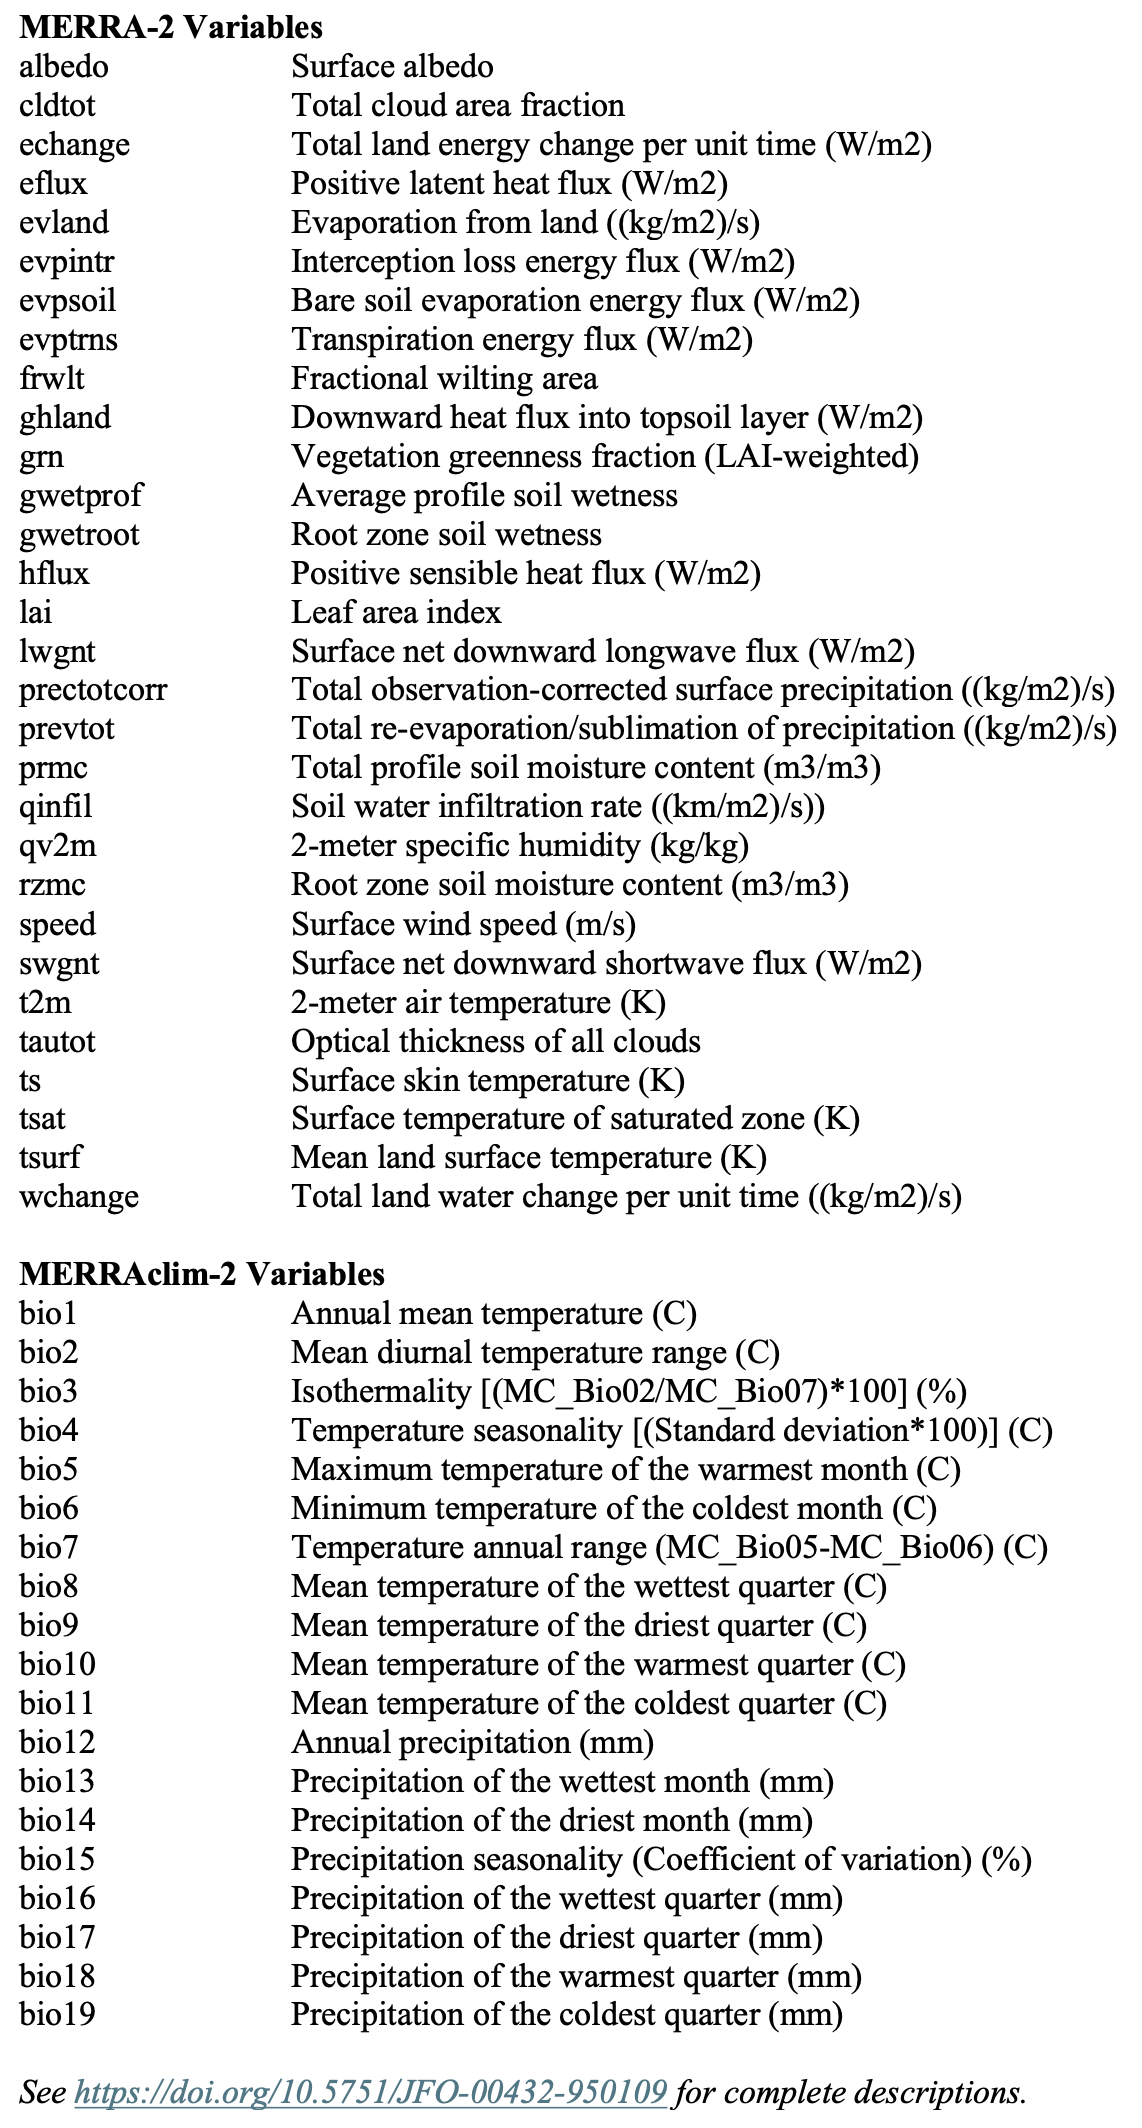
\includegraphics[width=4.02in,height=\textheight,keepaspectratio]{images/clipboard-2180550565.png}\hfill

\newpage{}

\section{APPENDIX C - Function
reference}\label{appendix-c---function-reference}

\subsubsection{rENM}\label{renm}

{\def\LTcaptype{none} % do not increment counter
\begin{longtable}[]{@{}
  >{\raggedright\arraybackslash}p{(\linewidth - 4\tabcolsep) * \real{0.3333}}
  >{\raggedright\arraybackslash}p{(\linewidth - 4\tabcolsep) * \real{0.3333}}
  >{\raggedright\arraybackslash}p{(\linewidth - 4\tabcolsep) * \real{0.3333}}@{}}
\toprule\noalign{}
\begin{minipage}[b]{\linewidth}\raggedright
Function
\end{minipage} & \begin{minipage}[b]{\linewidth}\raggedright
Description
\end{minipage} & \begin{minipage}[b]{\linewidth}\raggedright
See
\end{minipage} \\
\midrule\noalign{}
\endhead
\bottomrule\noalign{}
\endlastfoot
\texttt{rENM()} & Execute the complete rENM pipeline for a target
species & \emph{The rENM Workflow} \\
\end{longtable}
}

\subsubsection{rENM.core}\label{renm.core}

{\def\LTcaptype{none} % do not increment counter
\begin{longtable}[]{@{}
  >{\raggedright\arraybackslash}p{(\linewidth - 4\tabcolsep) * \real{0.3333}}
  >{\raggedright\arraybackslash}p{(\linewidth - 4\tabcolsep) * \real{0.3333}}
  >{\raggedright\arraybackslash}p{(\linewidth - 4\tabcolsep) * \real{0.3333}}@{}}
\toprule\noalign{}
\begin{minipage}[b]{\linewidth}\raggedright
Function
\end{minipage} & \begin{minipage}[b]{\linewidth}\raggedright
Description
\end{minipage} & \begin{minipage}[b]{\linewidth}\raggedright
See
\end{minipage} \\
\midrule\noalign{}
\endhead
\bottomrule\noalign{}
\endlastfoot
\texttt{rENM\_project\_dir()} & Resolve the active project root &
\emph{Configuring the RStudio Environment} \\
\texttt{get\_species\_info()} & Retrieve metadata for a species by alpha
code & \emph{Performing an rENM Analysis} \\
\texttt{show\_species()} & List species available in the project &
\emph{Performing an rENM Analysis} \\
\texttt{show\_variables()} & List environmental variables available in
the project & \emph{Data Assembly} \\
\end{longtable}
}

\subsubsection{rENM.data}\label{renm.data}

All functions in this package are documented in \emph{Data Assembly}.

{\def\LTcaptype{none} % do not increment counter
\begin{longtable}[]{@{}
  >{\raggedright\arraybackslash}p{(\linewidth - 2\tabcolsep) * \real{0.5000}}
  >{\raggedright\arraybackslash}p{(\linewidth - 2\tabcolsep) * \real{0.5000}}@{}}
\toprule\noalign{}
\begin{minipage}[b]{\linewidth}\raggedright
Function
\end{minipage} & \begin{minipage}[b]{\linewidth}\raggedright
Description
\end{minipage} \\
\midrule\noalign{}
\endhead
\bottomrule\noalign{}
\endlastfoot
\texttt{find\_occurrence\_extent()} & Derive spatial extent from
occurrence data \\
\texttt{find\_range\_extent()} & Derive spatial extent from a USGS GAP
range polygon \\
\texttt{get\_ebird\_occurrences()} & Read and bin an eBird EBD file into
five-year temporal bins \\
\texttt{get\_merra\_variables()} & Crop MERRA-2 predictor rasters to the
species extent \\
\texttt{limit\_record\_count()} & Downsample bins to a maximum record
count \\
\texttt{remove\_duplicate\_occurrences()} & Remove exact-coordinate
duplicate records \\
\texttt{set\_extent()} & Set spatial extent from explicit coordinates \\
\texttt{thin\_occurrences()} & Sequential spatial thinning \\
\texttt{thin\_occurrences2()} & Parallel spatial thinning with optional
record cap \\
\texttt{tidy\_occurrences()} & Move cleaned occurrence files from
staging to main directory \\
\end{longtable}
}

\subsubsection{rENM.model}\label{renm.model}

All functions in this package are documented in \emph{Time Series
Construction}.

{\def\LTcaptype{none} % do not increment counter
\begin{longtable}[]{@{}
  >{\raggedright\arraybackslash}p{(\linewidth - 2\tabcolsep) * \real{0.5000}}
  >{\raggedright\arraybackslash}p{(\linewidth - 2\tabcolsep) * \real{0.5000}}@{}}
\toprule\noalign{}
\begin{minipage}[b]{\linewidth}\raggedright
Function
\end{minipage} & \begin{minipage}[b]{\linewidth}\raggedright
Description
\end{minipage} \\
\midrule\noalign{}
\endhead
\bottomrule\noalign{}
\endlastfoot
\texttt{create\_ensemble\_model()} & Fit an ensemble ENM for a single
species and time bin \\
\texttt{create\_range\_map()} & Produce a binary presence-absence range
map \\
\texttt{create\_timeseries()} & Run ensemble models across all time bins
in parallel \\
\texttt{plot\_suitability()} & Plot a continuous climatic suitability
raster \\
\texttt{rank\_variable\_importance()} & Parse and rank variable
importance from an SDM model report \\
\texttt{reduce\_covariance()} & Remove collinear predictors via adaptive
VIF screening \\
\texttt{save\_suitability\_plot()} & Save a suitability plot to file \\
\texttt{screen\_by\_convergence1()} & Convergence-based variable
screening via MaxEnt (requires Java) \\
\texttt{screen\_by\_convergence2()} & Convergence-based variable
screening via maxnet (no Java dependency) \\
\texttt{stage\_all\_variables()} & Copy all predictor rasters into
TimeSeries bins \\
\texttt{stage\_occurrences()} & Copy occurrence files into TimeSeries
bins \\
\texttt{stage\_screened\_variables()} & Copy screened predictors into
TimeSeries bins \\
\end{longtable}
}

\subsubsection{rENM.analysis}\label{renm.analysis}

All functions in this package are documented in \emph{Time Series
Analysis}.

{\def\LTcaptype{none} % do not increment counter
\begin{longtable}[]{@{}
  >{\raggedright\arraybackslash}p{(\linewidth - 2\tabcolsep) * \real{0.5000}}
  >{\raggedright\arraybackslash}p{(\linewidth - 2\tabcolsep) * \real{0.5000}}@{}}
\toprule\noalign{}
\begin{minipage}[b]{\linewidth}\raggedright
Function
\end{minipage} & \begin{minipage}[b]{\linewidth}\raggedright
Description
\end{minipage} \\
\midrule\noalign{}
\endhead
\bottomrule\noalign{}
\endlastfoot
\texttt{analyze\_weighted\_centroids()} & Fit Bayesian trends to
centroid coordinates \\
\texttt{create\_hot\_spot\_map()} & Map hotspot regions within states
intersecting the GAP range \\
\texttt{create\_state\_trend\_analysis()} & Per-state suitability trend
map and statistics \\
\texttt{create\_suitability\_change\_map()} & Suitability rate-of-change
trend map \\
\texttt{find\_bioclimatic\_velocity()} & Estimate suitability
displacement direction, distance, and velocity \\
\texttt{find\_hot\_spots()} & Identify cells with accelerating
suitability declines \\
\texttt{find\_range\_change\_percentages()} & Summarize trend
proportions within the USGS GAP range \\
\texttt{find\_suitability\_change\_trend()} & Compute trends in
suitability rate of change \\
\texttt{find\_suitability\_trend()} & Compute per-cell Theil-Sen trends
and Mann-Kendall statistics \\
\texttt{find\_trend\_percentages()} & Summarize trend proportions across
the modeled extent \\
\texttt{find\_weighted\_centroid()} & Compute suitability-weighted
spatial centroids (called internally by
\texttt{analyze\_weighted\_centroids()}) \\
\texttt{gather\_variable\_contributions()} & Consolidate per-year
variable importance files \\
\texttt{plot\_suitability\_change\_trend()} & Plot suitability
rate-of-change trend raster \\
\texttt{plot\_trend()} & Plot a climatic suitability trend raster \\
\texttt{plot\_trend\_with\_centroids()} & Plot suitability trend with
centroid displacement overlay \\
\texttt{save\_trend\_plot()} & Save a suitability trend map to file \\
\texttt{save\_trend\_plot\_with\_centroids()} & Save a suitability trend
map with centroid displacement vector \\
\texttt{summarize\_variable\_contributions()} & Frequentist and Bayesian
trend analysis of variable contributions \\
\end{longtable}
}

\subsubsection{rENM.ai}\label{renm.ai}

All functions in this package are documented in \emph{GenAI Analysis}.

{\def\LTcaptype{none} % do not increment counter
\begin{longtable}[]{@{}
  >{\raggedright\arraybackslash}p{(\linewidth - 2\tabcolsep) * \real{0.5000}}
  >{\raggedright\arraybackslash}p{(\linewidth - 2\tabcolsep) * \real{0.5000}}@{}}
\toprule\noalign{}
\begin{minipage}[b]{\linewidth}\raggedright
Function
\end{minipage} & \begin{minipage}[b]{\linewidth}\raggedright
Description
\end{minipage} \\
\midrule\noalign{}
\endhead
\bottomrule\noalign{}
\endlastfoot
\texttt{assemble\_ai\_package()} & Assemble AI-ready data bundle with
analytical prompt \\
\texttt{render\_ai\_docx()} & Convert AI-generated DOCX report to PDF
via LibreOffice \\
\texttt{submit\_to\_chatgpt()} & Submit data bundle to OpenAI and
retrieve DOCX report \\
\texttt{submit\_to\_claude()} & Submit data bundle to Anthropic and
retrieve DOCX report \\
\texttt{submit\_to\_claude\_diag()} & Diagnose a failed
\texttt{submit\_to\_claude()} response \\
\end{longtable}
}

\subsubsection{rENM.reports}\label{renm.reports}

All functions in this package are documented in \emph{Report Generation}
and \emph{Assembling the Final Report}.

{\def\LTcaptype{none} % do not increment counter
\begin{longtable}[]{@{}
  >{\raggedright\arraybackslash}p{(\linewidth - 2\tabcolsep) * \real{0.5000}}
  >{\raggedright\arraybackslash}p{(\linewidth - 2\tabcolsep) * \real{0.5000}}@{}}
\toprule\noalign{}
\begin{minipage}[b]{\linewidth}\raggedright
Function
\end{minipage} & \begin{minipage}[b]{\linewidth}\raggedright
Description
\end{minipage} \\
\midrule\noalign{}
\endhead
\bottomrule\noalign{}
\endlastfoot
\texttt{assemble\_centroid\_trends\_page()} & Single-page PDF: centroid
trend map and table \\
\texttt{assemble\_final\_report()} & Combine all pages into a single
paginated PDF report \\
\texttt{assemble\_range\_timeseries\_page()} & Single-page PDF: range
time series contact sheet \\
\texttt{assemble\_state\_trends\_page()} & Single-page PDF: state trend
map, hotspot map, and table \\
\texttt{assemble\_suitability\_timeseries\_page()} & Single-page PDF:
suitability time series contact sheet \\
\texttt{assemble\_suitability\_trends\_page()} & Single-page PDF:
suitability trend and rate-of-change maps \\
\texttt{assemble\_variable\_trend\_maps\_page()} & Single-page PDF:
variable trend map composites \\
\texttt{assemble\_variable\_trends\_page()} & Single-page PDF: variable
contributions plot and table \\
\texttt{create\_centroid\_trend\_summary\_table()} & Centroid shift and
regression summary table \\
\texttt{create\_suitability\_trend\_summary\_table()} & State-level GAP
range and hotspot summary table \\
\texttt{create\_variable\_trend\_summary\_table()} & Variable trend
statistics summary table \\
\texttt{gather\_range\_maps()} & Assemble range map contact sheet \\
\texttt{gather\_suitability\_maps()} & Assemble suitability map contact
sheet \\
\texttt{gather\_suitability\_trend\_stats()} & Merge state-level
suitability and hotspot statistics \\
\texttt{gather\_top\_variable\_trend\_maps()} & Assemble variable trend
map composites \\
\end{longtable}
}




\end{document}
